%%% Local Variables:
%%% mode: latex
%%% TeX-master: t
%%% End:

\documentclass[bachelor,winfonts]{thuthesis}
%\documentclass[master]{thuthesis}
%\documentclass[doctor]{thuthesis}
% \documentclass[%
%   bachelor|master|doctor|postdoctor, % mandatory option
%   winfonts|nofonts|adobefonts, % mandatory only for bachelor and Linuxer
%   secret,
%   openany|openright,
%   arialtoc,arialtitle]{thuthesis}
% 当使用 XeLaTeX 编译时,本科生、Linux 用户需要加上 nofonts 选项;
% 当使用 PDFLaTeX 编译时,adobefonts 选项等效于 winfonts 选项(缺省选项)。

% 所有其它可能用到的包都统一放到这里了,可以根据自己的实际添加或者删除。
\usepackage{thutils}

% 你可以在这里修改配置文件中的定义,导言区可以使用中文。
% \def\myname{薛瑞尼}

\begin{document}

% 定义所有的eps文件在 figures 子目录下
\graphicspath{{figures/}}


%%% 封面部分
\frontmatter

%%% Local Variables:
%%% mode: latex
%%% TeX-master: t
%%% End:
\secretlevel{} \secretyear{}

\ctitle{通过 RNA-Seq 估计转录本长度和辨识剪切异构体的研究}
% 根据自己的情况选,不用这样复杂
\makeatletter
\ifthu@bachelor\relax\else
  \ifthu@doctor
    \cdegree{工学博士}
  \else
    \ifthu@master
      \cdegree{工学硕士}
    \fi
  \fi
\fi
\makeatother


\cdepartment[自动化]{自动化系}
\cmajor{自动化}
\cauthor{李天阳} 
\csupervisor{张学工}
% 如果没有副指导老师或者联合指导老师,把下面两行相应的删除即可。
\cassosupervisor{江瑞}
% 日期自动生成,如果你要自己写就改这个cdate
%\cdate{\CJKdigits{\the\year}年\CJKnumber{\the\month}月}

% 博士后部分
% \cfirstdiscipline{计算机科学与技术}
% \cseconddiscipline{系统结构}
% \postdoctordate{2009年7月——2011年7月}

\etitle{Research on using RNA-Seq to estimate transcript length and identify isoforms} 
% 这块比较复杂,需要分情况讨论:
% 1. 学术型硕士
%    \edegree:必须为Master of Arts或Master of Science(注意大小写)
%              “哲学、文学、历史学、法学、教育学、艺术学门类,公共管理学科
%               填写Master of Arts,其它填写Master of Science”
%    \emajor:“获得一级学科授权的学科填写一级学科名称,其它填写二级学科名称”
% 2. 专业型硕士
%    \edegree:“填写专业学位英文名称全称”
%    \emajor:“工程硕士填写工程领域,其它专业学位不填写此项”
% 3. 学术型博士
%    \edegree:Doctor of Philosophy(注意大小写)
%    \emajor:“获得一级学科授权的学科填写一级学科名称,其它填写二级学科名称”
% 4. 专业型博士
%    \edegree:“填写专业学位英文名称全称”
%    \emajor:不填写此项
\edegree{Bachelor of Engineering} 
\emajor{Automation} 
\eauthor{Li Tianyang} 
\esupervisor{Zhang Xuegong} 
\eassosupervisor{Jiang Rui} 
% 这个日期也会自动生成,你要改么?
% \edate{December, 2005}

% 定义中英文摘要和关键字
\begin{cabstract}
	RNA-Seq 是最近几年发展起来的通过高通量测序对转录组中的序列进行测序的一种技术。 
	RNA-Seq 技术的发展使得人们在最近几年当中对于生物中的基因表达的规律, 
	以及基因组上的功能模块有了更为深入的了解。 
	在通过 RNA-Seq 数据确定基因的表达量时, 我们需要知道基因序列的长度。 
	但是在没有基因注释或者没有基因组参考序列时, 我们需要一种得知基因的长度的方法。
	本文提出了一个通过 RNA-Seq 数据对转录本的长度进行估计的统计方法。 
	通过该方法, 我们可以在基因组参考序列没有基因注释信息, 以及没有基因组参考序列, 
	的情况下使用 RNA-Seq 数据估计出转录本的长度。
	同时, 在 RNA-Seq 数据中我们发现读段的分布位置不均匀。
	此处我们对 RNA-Seq 数据中读段分布的不均匀性做了初步的分析。
	此外, 真核生物的基因在有多个外显子的情况下会有选择性剪切的现象发生, 
	同一个基因可能会产生多个剪切异构体。
	通过 RNA-Seq 数据我们可以辨别一个基因的不同的剪切异构体。
	本文证明了用最大似然的方法通过真核生物 RNA-Seq 数据辨识基因的剪切异构体是一个 NP 难问题。
\end{cabstract}

\ckeywords{RNA-Seq, 转录组, 转录本}

\begin{eabstract} 
	RNA-Seq is a technology developed in the last few years for sequencing the transcriptome using high throughput sequencing. 
	Using RNA-Seq, people have gained much deeper understanding of gene expression patterns, 
	and functional modules in genomes. 
	When estimating a transcript's expression level with RNA-Seq, 
	we need to know the length of the transcript's sequence. 
	However, when no annotations or reference genome sequences are available, 
	we need another method to know the transcript's length. 
	Here, we present a statistical method to estimate transcript length using RNA-Seq. 
	Using this method, we can estimate a transcript's length when no annotations are available for the reference genome sequences, or when the reference genome sequences are not available. 
	We also observed that RNA-Seq reads are non-uniformly distributed. 
	Here, we present a preliminary analysis on the non-uniform distribution of RNA-Seq reads. 
	And it has been observed in eukaryotes a gene with multiple exons can correspond to multiple isoforms due to alternative splicing. With RNA-Seq, we can determine a gene's isoroms. 
	Here, we prove that using eukaryotic RNA-Seq data to identify a gene's isoforms by maximum likelihood is NP-hard.
\end{eabstract}

\ekeywords{RNA-Seq, transcriptome, transcript}




% 设置 PDF 文档的作者、主题等属性
\makeatletter
\thu@setup@pdfinfo
\makeatother
\makecover

% 目录
\tableofcontents

% 符号对照表
\begin{denotation}

\item[HPC] 高性能计算 (High Performance Computing)

\end{denotation}



%%% 正文部分
\mainmatter
\chapter{引言}

\section{RNA-Seq}
\nocite{wang2009rna, ozsolak2010rna}

RNA-Seq 是对 RNA 序列进行测量的一种技术, 
它是近几年来发展起来的通过深度测序用于研究转录组的一种技术. 
与其他的方法相比起来, RNA-Seq 揭露了生物的转录组中更多的复杂性. 
同时, RNA-Seq 能够更好地研究生物的转录组中各转录本的表达量. 
通过了解细胞中在某种特定条件下转录组中的转录本的组成, 
以及每一个转录本的表达量, 我们可以了解基因上的不同的功能模块, 
进而了解生物的发育过程, 以及疾病与人体之间的关系. 
通过使用 RNA-Seq, 我们已经对编码蛋白质的基因以及它们的剪切异构体 (isoform) 有了更为深入的了解. 
此外, RNA-Seq 也帮助我们对于基因上的非编码区域有了更为深入的认识, 
例如 lncRNA (long non-coding RNA).
并且我们对 sRNA (small RNA), microRNA 等也有了更全面的了解. 
\cite{pickrell2010understanding, encode, nagalakshmi2008transcriptional, 
tang2009mrna, banfai2012long, mortazavi2008mapping, wang2008alternative, 
katz2010analysis, deng2011isoform, lu2010function, mercer2011targeted, 
howald2012combining, lalonde2011rna, djebali2012landscape, 
derrien2012gencode, gerstein2012architecture, fairfax2012genetics, 
morrissy2011extensive, howald2012combining, park2012rna, 
tilgner2012deep, orom2010long, mercer2011human, chung2011computational, 
gingeras2009implications, roy2010identification, axtell2011vive, 
berezikov2010evolutionary, cherbas2011transcriptional, anders2012detecting, 
stoeckius2009large, lau2009abundant}

在 RNA-Seq 技术出现之前, 人们主要通过微阵列 (microarray) 对转录组进行定量分析和研究 \cite{schena1995quantitative}. 
但是与 RNA-Seq 相比, 微阵列存在若干问题 \cite{wang2009rna}: 
\begin{itemize}
\item 微阵列只能在序列已知的情况下使用

\item 结果会受交叉杂交 (cross-hybridization) 影响 \cite{okoniewski2006hybridization, royce2007toward}

\item 测量的表达量范围有限
\end{itemize}
另外, 在 RNA-Seq 技术出现之前, 人们主要通过 Sanger 测序法对互补 DNA (cDNA) 序列或者表达序列标签库 (EST libraries) 进行测序来研究转录组的序列 \cite{boguski1994gene, gerhard2004status}. 
但是 Sanger 测序价格昂贵, 同时测序通量偏低, 无法对转录组进行定量分析和研究. 
高通量测序技术的发展使得我们能够在较短的时间内用较少的成本对大量序列进行测序, 
几乎完整地测量转录组的序列, 
同时建立测序数量和实际被测序分子的数量间的关系 \cite{marioni2008rna}. 
这些是 RNA-Seq 在当今被广泛应用的一个主要原因. 

\begin{figure}[!t]
\centering
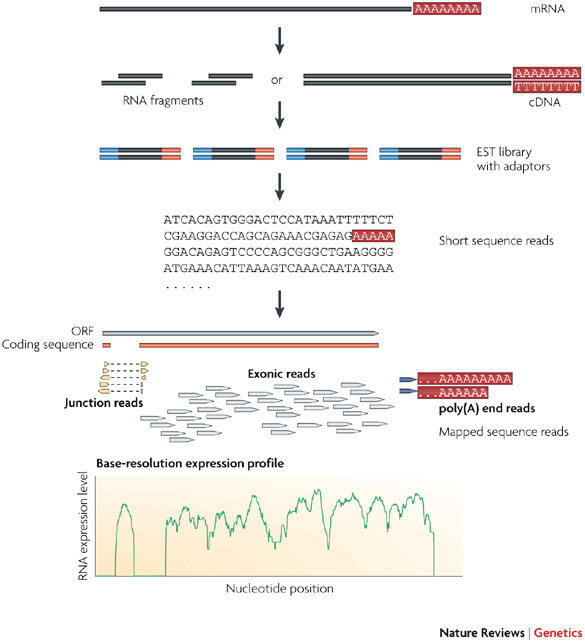
\includegraphics[width=\textwidth]{figures/rna-seq-experiment.jpg}
\caption{一般的 RNA-Seq 实验流程 \cite{wang2009rna}}
\label{intro-rna-seq-ex}
\end{figure}

\section{RNA-Seq 数据分析方法简介}
RNA-Seq 通常直接用于对于这些生物问题的研究:
\begin{itemize}
\item 发现新的剪切异构体 \cite{merkin2012evolutionary, wang2010novo, roberts2011identification, wang2010mapsplice}

\item 研究 RNA 序列的对于生物的调控作用 \cite{van2011xuts}

\item 比较不同条件下转录组不同的构成 \cite{trapnell2012differential}
\end{itemize}
同时, RNA-Seq 数据还未研究其他生物问题提供了宝贵的原始数据, 
例如对于生物系统中的网络的研究 \cite{sinicropi2012whole}. 

为了能够通过 RNA-Seq 数据对生物问题有深入的研究, 
我们通常会对 RNA-Seq 数据用这些方法进行处理:
\begin{itemize}
\item 序列比对 (sequence alignment): 将 RNA-Seq 读段找到其在基因组中的位置

\item 序列拼装: 
直接将 RNA-Seq 读段拼装成原转录组的各转录本. 若拼装时不依赖已知的参考序列, 
则成为 \textit{de novo} 拼装 ((\textit{de novo} assembly)). 

\item 转录本的表达量估计: 用一定的单位表示每个被测样本中转录组里每个转录本的含量, 
用于在不同的样本之间进行比较

\item 辨识同一个基因的剪切异构体 (真核生物 RNA-Seq 数据): 真核生物中由于选择性剪切同一个基因会产生多个剪切异构体, 
通过 RNA-Seq 数据在一定条件下可以辨识出一个基因的不同的剪切异构体
\end{itemize}

\subsection{序列比对}
经典的序列比对算法包括 Smith-Waterman 算法 \cite{SmithWaterman1981} 和 Needleman-Wunsch 算法 \cite{needleman1970general}. 
但是由于 Smith-Waterman 算法和 Needleman-Wunsch 算法复杂度偏高, 它们不适用于大规模的数据. 
目前人们一般采用一些启发式的方法进行序列比对 \cite{isaev2004introduction}. 
对于将 RNA-Seq 读段比对到其在基因组中的位置, 目前比较常用的工具包括: 
\begin{itemize}
\item BLAT \cite{kent2002blat}
\item TopHat \cite{trapnell2009tophat}
\end{itemize}

\subsection{序列拼装}
序列拼装是生物信息学和计算生物学中一个经典的问题, 
其目的是通过测序的读段恢复出原始的生物序列. 对于序列拼装, 目前人们主要采用一下这两种常用的策略: 
\begin{itemize}
\item OLC (overlap-layout-consensus) \cite{greenphrap, bonfield1995new, 
kececioglu1995combinatorial, myers1995toward, huang1999cap3}

\item de Bruijn 图 \cite{pevzner2001eulerian}
\end{itemize}
目前对于 RNA-Seq 数据的拼装主要有这些常用的工具: 
\begin{itemize}
\item Cufflinks \cite{cufflinks.2010}: 
OLC 策略 (图 \ref{intro-cufflinks-assembly})

\item Trinity \cite{grabherr2011full}: 
de Bruijn 图策略 (图 \ref{intro-trinity-assembly})
\end{itemize}

\begin{figure}[!t]
\centering
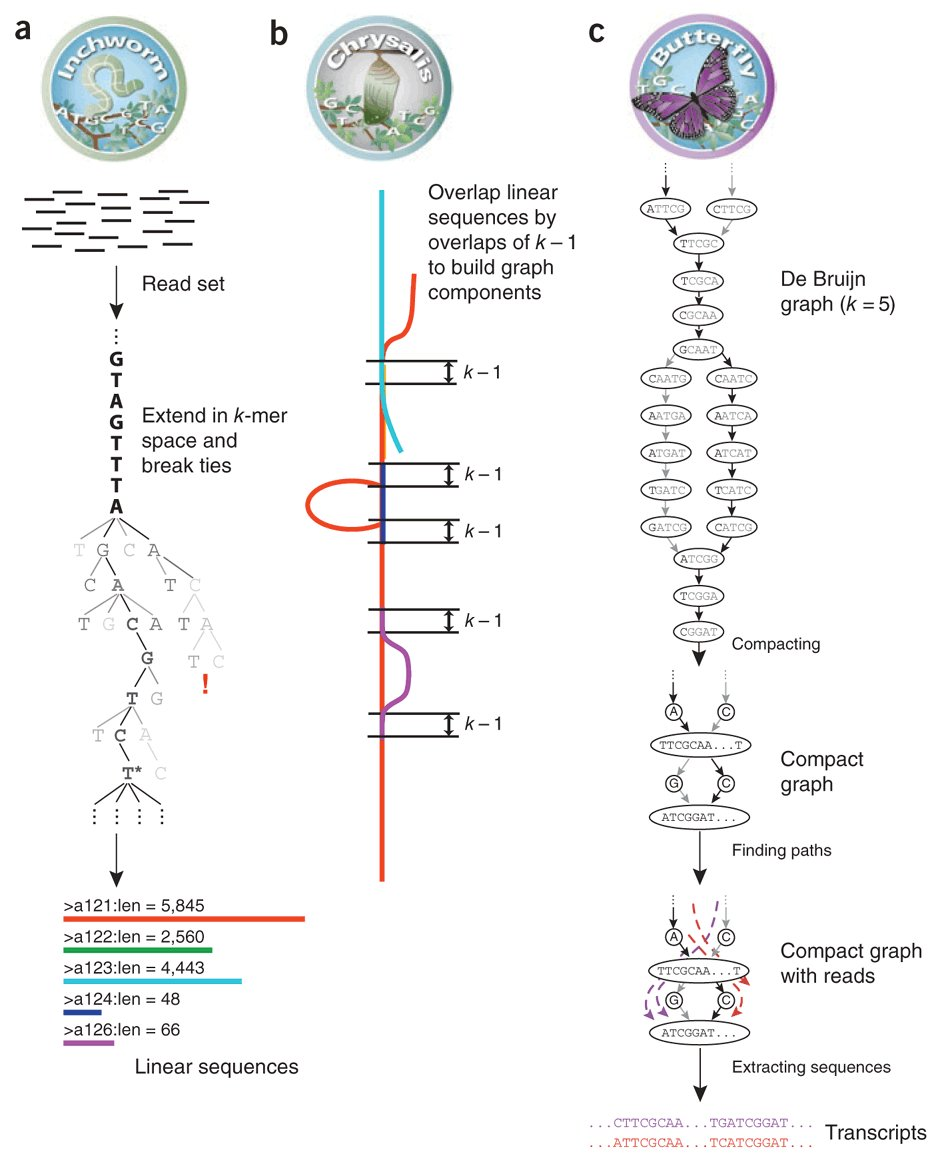
\includegraphics[width=\textwidth]{figures/trinity-assembly.jpg}
\caption{Trinity 拼装策略 \cite{grabherr2011full}}
\label{intro-trinity-assembly}
\end{figure}

\subsection{转录本的表达量估计}
通过量化转录组中各转录本, 从实验数据中估计其表达量, 
我们可以对生物系统中的结构和过程有更好的量化的认识. 
RNA-Seq 技术的发展对于转录本表达量的估计有很大的帮助. 
在 RNA-Seq 实验中, 
通常使用 RPKM (reads per kilobase per million reads sequenced) 
\cite{mortazavi2008mapping} 作为一个转录本表达量的单位. 
目前在 RNA-Seq 实验中通常使用的转录本表达量估计的工具包括: 
\begin{itemize}
\item Cufflinks \cite{cufflinks.2010} (图 \ref{intro-cufflinks-abundance})
\end{itemize}

\begin{figure}[!t]
\centering
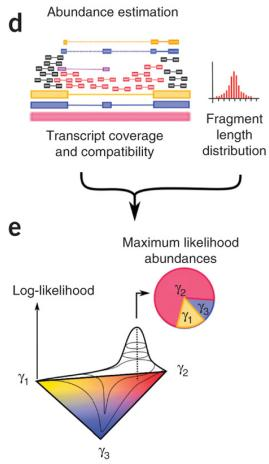
\includegraphics[height=0.5\textheight]{figures/cufflinks-abundance.jpg}
\caption{Cufflinks 对转录本的表达量的估计 \cite{cufflinks.2010}}
\label{intro-cufflinks-abundance}
\end{figure}

\subsection{辨识同一个基因的剪切异构体 (真核生物 RNA-Seq 数据)}
经过多年的研究, 人们认识到真核生物的同一个基因会有多个剪切异构体 
\cite{gilbert1978genes, rosenfeld1982calcitonin, early1980two, 
citeulike:447573, modrek2002genomic}. 
RNA-Seq 技术的发展大大促进了人们对于真核生物中选择性剪切的认识, 
因为 RNA-Seq 数据可以较好地表现出来真核生物中的选择性剪切的现象. 
目前在真核生物相关的 RNA-Seq 实验中通常使用的用于辨识同一个基因的剪切异构体的工具包括: 
\begin{itemize}
\item Cufflinks \cite{cufflinks.2010} (图 \ref{intro-cufflinks-assembly})
\end{itemize}

\begin{figure}[!t]
\centering
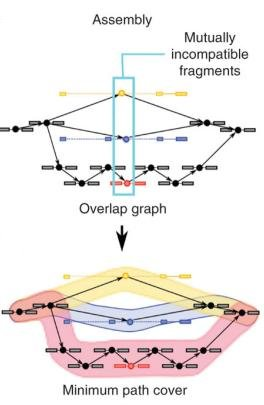
\includegraphics[height=0.5\textheight]{figures/cufflinks-assembly.jpg}
\caption{Cufflinks 序列拼装策略和对同一个基因的剪切异构体的辨识 \cite{cufflinks.2010}}
\label{intro-cufflinks-assembly}
\end{figure}

\section{现有 RNA-Seq 数据定量分析方法}

\subsection{RNA-Seq 数据定量分析的一般模型}
\label{rna-seq-general-model}

\onlinecite{2011arXiv1104.3889P} 对RNA-Seq 数据定量分析建立了一个一般的模型, 
用统计的方法对 RNA-Seq 数据进行定量分析. 在这里我们对这个模型进行介绍. 

下面是为了描述该模型所使用的一些符号, 以及一些假设: 
\begin{itemize}
\item $G$ 表示转录组中所有包含的基因所组成的集合.

\item $I_g$, $g \in G$ 表示基因 $g$ 在转录组中所有的剪切异构体组成的集合, 
$I = \bigcup_{g \in G} I_g$ 是所有的剪切异构体所构成的集合. 
此处为了方便描述, 我们也将无选择性剪切的基因所对应的转录本称作是它的剪切异构体. 

\item $q(p, i)$ 表示对于一个剪切异构体 $i \in I$, 
来自 $i$ 的一个读段 (read) 或片段 (fragment) 的起始位置 (5' 段) 是 $p$ 的概率. 
对于给定的一个剪切异构体 $i$, 
$\sum_{p \in \{ \text{所有读段或片段起始位置} \}} q(p, i) = 1$. 

\item 所有读段或片段构成的集合表示为 $R$ 

\item 所有的读段或片段都是独立的. 

\item 当给定一个剪切异构体 $i$ 和它上面一个读段或片段的起始位置 $p$ 时, 
$q(p, i)$ 是已知的. 

\item 一个读段或片段 $r \in R$ 可以是来自多个 $I$ 中的剪切异构体, 
但是给定一个剪切异构体 $i$, 
用序列比对的方法将 $r$ 比对到 $i$ 上的所有位置是唯一的. 
对于基因序列的分析表明这样一个假设是合理的 \cite{peng2011t}. 
\end{itemize}















\chapter{通过 RNA-Seq 数据估计转录本的长度}
\label{chap-lenest}

\section{介绍}
在这里我们介绍一个能够通过 RNA-Seq 数据在没有已知基因注释的情况下估计一个转录本的长度的统计方法. 

对于目前大部分现有的 RNA-Seq 数据, 
我们都无法直接从数据中直接获得其所包含的转录本在基因组上的 5' 段和 3' 段的位置. 
但是在 RNA-Seq 实验中为了能够测量每一个转录本的表达量, 
我们在计算其表达量时均需要使用到该转录本的长度 
\cite{mortazavi2008mapping, Jiang15042009, cufflinks.2010}. 
在使用基因组及其所对应的基因注释的情况下 (例如 RefSeq \cite{_refseq}), 
在分析时可以直接采用注释中的基因位置得出各转录本的长度. 
在没有基因注释, 或者在没有基因组参考序列的情况下, 
如果不采用更加复杂的技术, 如 RNA-PET \cite{Fullwood01042009} 技术, 
则需要通过 RNA-Seq 数据估计出转录本的长度. 对于现有的大部分 RNA-Seq 数据, 
仍然没有对应的 RNA-PET 数据用语确定各转录本的 5' 和 3' 段. 
所以对于通过 RNA-Seq 数据直接估计转录本的长度是有需求的. 

\section{理论分析}
在通过 RNA-Seq 数据估计转录本的时候我们对 RNA-Seq 数据做如下的假设以简化模型: 
\begin{itemize}
\item 所有的读段在原转录本上的位置的分布都是独立的. 

\item 所有的读段的长度都是相同的, 为 $R$ bp 长.

\item 读段的 5' 段位置 (以下称之为起始位置) 在原转录本上的分布是均匀的. 
同样的, 读段的 3' 段位置 (以下称之为终止位置) 在原转录本上的分布也是均匀的. 
\end{itemize}

为了在基因组参考序列没有基因注释, 甚至于没有基因组参考序列, 
的情况下能够通过 RNA-Seq 数据估计出转录本的长度, 
我们在这里给出定理 \ref{len-est-thm-one-end} 和 
定理 \ref{len-est-thm-2-ends} 及其证明. 
通过定理 \ref{len-est-thm-one-end} 和 
定理 \ref{len-est-thm-2-ends} 
我们可以通过 RNA-Seq 数据估计出转录本的长度. 
在这里建议读者参考 \onlinecite{casella2002statistical} 
和 \onlinecite{ewens2005statistical}. 

\begin{thm}
\label{len-est-thm-one-end}
假设 $X_1$, $X_2$, \ldots, $X_N$ 是来自定义在 
${1, 2, \ldots , L}$, $L \in \mathbb{Z}^+$ 的均匀分布, 
即 
\[
P(X = i) =  \begin{cases}
\frac{1}{L} & \text{ 当 } 1 \leq i \leq L \\
0 & \text{ 其余情况 }
\end{cases}
\]
则对于 $L$ 的最小方差无偏估计 $\hat{L}$ 为
\begin{equation}
\label{len-est-thm-on-end-eq}
\hat{L} = \frac{ {X_{(N)}}^{N+1} - (X_{(N)} - 1)^{N+1} }{ {X_{(N)}}^N - (X_{(N)} - 1)^N }
\end{equation}
其中 $X_{(N)} = \max_{1 \leq i \leq N} X_i$. 
\end{thm}

通过定理 \ref{len-est-thm-one-end} 我们可以在已知转录本上一个固定的位点 
(例如外显子出现剪切现象的边界), 根据读段的起始位置 (或者终止位置), 
估计出着一个位于转录本上的固定的位点到转录本的一端的序列的长度, 
从而能够估计出转录本的长度. 

下面我们给出定理 \ref{len-est-thm-one-end} 的证明. 

\begin{proof}
我们首先说明 
\[
X_{(N)} = \max_{1 \leq i \leq N} X_i
\] 
在定理中的假设下是一个充分统计量. 

由于在这里考虑的是一个离散的均匀分布, 我们容易注意到
\[
P(X_1, X_2, \ldots, X_N | X_{(N)}) = \frac{1}{ {X_{(N)}}^N - (X_{(N)} - 1)^N }
\]
与该分布的参数 $L$无关, 所以 $X_{(N)}$ 是一个充分统计量. 

另外, 根据离散的均匀分布的性质我们可以得到
\[
P(X_{(N)} = i) = \frac{ i^N - (i - 1)^N }{L^N}
\]

对于定理 \ref{len-est-thm-one-end} 中给出的估计 $\hat{L}$ 
(式 \eqref{len-est-thm-on-end-eq}), 
我们可以进一步计算 $\operatorname{E}[\hat{L}]$ 得
\begin{align*}
\operatorname{E}[\hat{L}] &= \sum_{i=1}^L P(X_{(N)} = i) 
    \frac{i^{N+1} - (i-1)^{N+1}}{i^N-(i-1)^{N-1}} \\
&= L
\end{align*}
从而我们可以知道定理 \ref{len-est-thm-one-end} 中给出的估计 $\hat{L}$ 
(式 \eqref{len-est-thm-on-end-eq}) 是无偏的. 

下面我们说明 $X_{(N)}$ 是一个完全统计量. 
即对于所有的 $L \in \mathbb{Z}^+$, 若有一个函数 $g(x)$, $x \in \mathbb{Z}^+$ 使得
\[
\operatorname{E}[g(X_{(N)})] = 0
\]
则 $g(x) = 0$ 对所有 $x \in \mathbb{Z}^+$ 成立. 

注意到
\[
\operatorname{E}[g(X_{(N)})] = 0
\]
对所有的 $L \in \mathbb{Z}^+$ 成立意味着
\begin{align*}
\frac{1^N - 0^N}{1^N} g(1) &= 0 \\
\frac{1^N - 0^N}{2^N} g(1) + \frac{2^N - 1^N}{2^N} g(2) &= 0 \\
\frac{1^N - 0^N}{3^N} g(1) + \frac{2^N - 1^N}{3^N} g(2) + \frac{3^N - 2^N}{3^N} g(3) &= 0 \\
\ldots
\end{align*}
所以根据数学归纳法, 我们容易得出 $g(x) = 0$ 对所有 $x \in \mathbb{Z}^+$ 成立. 
进而我们可以知道 $X_{(N)}$ 是一个完全统计量. 

由以上的分析我们知道: 
\begin{itemize}
\item $X_{(N)}$ 是一个充分统计量
\item $X_{(N)}$ 是一个完全统计量
\item 定理 \ref{len-est-thm-one-end} 中给出的估计 $\hat{L}$ 
(式 \eqref{len-est-thm-on-end-eq}) 对于此处的分布的参数 $L$ 的估计是无偏的 
\end{itemize}
从而根据 Lehmann-Scheff{\'e} 定理
\cite{lehmann2012completeness.p1, lehmann2012completeness.p2} 
我们可以得出定理 \ref{len-est-thm-one-end} 中给出的估计 $\hat{L}$ 
(式 \eqref{len-est-thm-on-end-eq}) 是对该分布的参数 $L$ 的最小方差无偏估计. 
\end{proof}

\begin{thm}
\label{len-est-thm-2-ends}
假设$X_1$, $X_2$, \ldots, $X_N$ 是来自定义在 
${p+1, p+2, \ldots , p+L}$, $p \in \mathbb{Z}$, $L \in \mathbb{Z}^+$ 的均匀分布, 
即 
\[
P(X = i) =  \begin{cases}
\frac{1}{L} & \text{ 当 } p+1 \leq i \leq p+L \\
0 & \text{ 其余情况 }
\end{cases}
\]
则对于 $L$ 的一个无偏估计 $\hat{L}$ 为
\begin{equation}
\label{len-est-thm-2-ends-eq}
\hat{L} = \frac{ D^{N+1} - 2 (D-1)^{N+1} + (\max(D-2, 0))^{N+1} }{ D^{N} - 2 (D-1)^{N} + (\max(D-2, 0))^{N} }
\end{equation}
其中 $D = \max_{1 \leq i \leq N} X_i - \min_{1 \leq i \leq N} X_i +1$. 
\end{thm}

通过定理 \ref{len-est-thm-2-ends} 我们可以在转录本上无法找到一个固定的位点时, 
通过 RNA-Seq 数据对转录本的长度进行估计. 
这种情况适用于在一个基因没有出现选择性剪切的现象时估计该转录本的长度, 
例如真核生物中只有一个外显子的基因或者是原核生物中的单个操纵子. 

下面我们给出定理 \ref{len-est-thm-2-ends} 的证明. 

\begin{proof}
根据均匀分布的性质, 我们容易得到
\[
P(D=i) = (L-D +1) \frac{ D^N - 2 (D-1)^N  + (\max(D-2,0))^N}{ L^N }
\]

从而
\begin{align*}
\operatorname{E}[\hat{L}] &= \sum_{i=1}^L P(D=i) 
    \frac{i^{N+1}-2(i-1)^{N+1}+(\max(i-2,0))^{N+1}}{i^N-2(i-1)^N+(\max(i-2,0))^N} \\
&= \frac{1}{L^N} \sum_{i=1}^L (L-i+1)(i^{N+1}-2(i-1)^{N+1}+(\max(i-2,0))^{N+1}) \\
&= L
\end{align*}
\end{proof}

下面我们介绍一个方法, 
通过这个方法我们可以在没有参考基因组序列的情况下从拼装的所有连续段 (contig) 
中挑选出覆盖原先转录本部分较多 (例如该连续段是该转录本唯一的一个连续段) 的连续段. 
因为在没有参考基因组序列的情况下, 若要认为一个连续段代表原基因, 
则必须要求该连续段覆盖了原转录本的大部分的区域. 
如果一个转录本的测序深度偏低, 覆盖低, 
则通过测序的结果我们可能看到这个转录本会拥有多个连续段, 
这样的情况在没有参考序列时是几乎无法分析的. 

我们在这里对此进行分析, 首先我们定义测序的覆盖 (coverage) $c$
\begin{equation}
c = \frac{NR}{L}
\end{equation}
其中 $R$ 是测序读段的长度, $N$ 是转录本上测序时得到的读段的个数, 
$L$ 是转录本的有效长度 ($\text{转录本实际长度} -R+1$). 

同时, 我们在这里介绍一个用来描述测序过程的 Poisson 模型. 
这里假设我们有一个无限长的序列, 
每一个位置上起始的读段个数都是一个参数为 $\lambda$ 的 Poisson 分布. 
并且所有位置的起始的读段个数均是独立的. 
在这里测序的覆盖和 $\lambda$ 的在理想的情况下满足如下的关系
\[
\lambda = c R
\]

当两个读段至少有一个碱基对重合时, 
我们认为这两个读段能够连接到一起组成一个更长的连续段. 通过这样的过程, 
我们将若干读段连接在一起构成连续段. 

为了挑选覆盖原转录本 ``较多'' 的连续段, 
我们在上面所述的测序模型下对每一个连续段考虑如下的一个概率
\begin{equation}
\label{lenest-one-contig-one-isof-prob-decription}
P(\text{观察到一个连续段其长度} \leq \text{目前的连续段 } |\text{ 目前的连续段的覆盖})
\end{equation}

为了更深入地了解式 \eqref{lenest-one-contig-one-isof-prob-decription} 中的概率, 
我们在这里分析
\begin{equation}
\label{lenest-one-cont-prob-distr}
P(\text{连续段长度} = l | \text{目前的连续段的覆盖} \lambda)
\end{equation}
即给定覆盖, 连续段的长度的分布. 
下面为方便讨论我们记
\begin{equation}
p_n =  \frac{P(\text{连续段长度} = n+R-1 | \text{目前的连续段的覆盖} \lambda)}{e^{-(R-1)\lambda}}
\end{equation}
则
\begin{align}
p_n &= 0 & n &\leq 0 \\
p_1 &= 1 & & \\
p_{n+R} &= \sum_{i=1}^{R-1} (1-e^{-\lambda}) e^{-(R-1-i)\lambda} p_{n+i} & n &\geq 2-R
\end{align}

为了估计式 \eqref{lenest-one-contig-one-isof-prob-decription} 中的概率, 
在这里我们先介绍一个改进的 Lander-Waterman 公式 (定理 \ref{discrete-lander-waterman}), 
原先的 Lander-Waterman 公式 \cite{lander1988genomic} 在推导中使用了一些近似, 
在这里我们不使用 \onlinecite{lander1988genomic} 中所使用的近似. 

\begin{thm}[改进的 Lander-Waterman 公式]
\label{discrete-lander-waterman-thm}
在之前的 Poisson 模型下, 一个连续段的期望的长度
\begin{equation}
\label{discrete-lander-waterman-formula}
\operatorname{E}[\text{一个连续段的长度}] = \frac{e^{R\lambda} - 1}{e^\lambda - 1} 
\end{equation}
\end{thm}

下面我们给出定理 \ref{discrete-lander-waterman-thm} 的证明. 

\begin{proof}
这里为了描述的1简便, 我们记
\begin{align*}
q &= 1 - e^{-\lambda} \\
1-q &= e^{-\lambda}
\end{align*}

为了证明定理 \ref{discrete-lander-waterman-thm} 
中的式 \eqref{discrete-lander-waterman-formula}, 
我们考虑相邻的读段起始位置的个数 $N_D$ (即两个位置是相邻的两个读段起始位置, 
同时这两个位置上的读段连接在了一起), 
以及两个相邻的有读段的位置间的差值 $D_i$, $i=1,2,\ldots,N_D$ 
(即用 $X_1=1,X_2,\ldots,X_{N_D}, X_{N_D+1}$ 表示若干个相邻的读段起始位置时, 
$D_i=X_{i+1}-X_i$, $i=1,2,\ldots,N_D$). 
根据这里所使用的模型, 我们容易知道 $D_i$, $i=1,2,\ldots,N_D$ 是 i.i.d. 

所以我们容易看出来
\begin{align*}
\operatorname{E}[\text{一个连续段的长度}] &= \operatorname{E}[X_{N_D + 1}] +R-1 \\
&= \operatorname{E}[\sum_{i=1}^{N_D} D_i] +R \\
&= \operatorname{E}[\operatorname{E}[\sum_{i=1}^{N_D} D_i|N_D]] +R \\
&= \operatorname{E}[D] \operatorname{E}[N_D] +R
\end{align*}

下面我们分别计算
\begin{align*}
\operatorname{E}[D] \\
\operatorname{E}[N_D]
\end{align*}
\end{proof}

\section{仿真分析}
XXX

\section{实际 RNA-Seq 数据分析}





%%% 其它部分
\backmatter

% 本科生要这几个索引,研究生不要。选择性留下。
\makeatletter
\ifthu@bachelor
  % 插图索引
  \listoffigures
  % 表格索引
  \listoftables
  % 公式索引
  \listofequations
\fi
\makeatother


% 参考文献
\bibliographystyle{thubib}
\bibliography{ref/refs}


% 致谢
%%% Local Variables:
%%% mode: latex
%%% TeX-master: "../main"
%%% End:

\begin{ack}
	衷心感谢导师张学工教授和江瑞副教授对本人的精心指导。 
	
	同时也感谢 \href{https://github.com/xueruini/thuthesis}{\thuthesis}, 
	以及其他各种开源项目给予我的帮助和支持。 
\end{ack}


% 附录
%\begin{appendix}
%%%% Local Variables: 
%%% mode: latex
%%% TeX-master: "../main"
%%% End: 

\chapter{源代码}
\begin{itemize}
\item \url{https://github.com/tianyang-li/de-novo-rna-seq-quant-1}
\item \url{https://github.com/tianyang-li/thu-undegrad-thesis-code}
\item \url{https://github.com/tianyang-li/aarsa}
\item \url{https://github.com/tianyang-li/rna-seq-len-est-0}
\item \url{https://github.com/tianyang-li/misc-bioinfo-0}
\item \url{https://github.com/tianyang-li/de-novo-metatranscriptome-analysis--the-uniform-model}
\item \url{https://github.com/tianyang-li/human-rna-seq-analysis-0}
\item \url{https://github.com/tianyang-li/de-novo-rna-seq-quant-with-contigs-py-0}
\item \url{https://github.com/tianyang-li/bi-misc}
\item \url{https://code.google.com/p/meta-transcriptome/}
\end{itemize}


%\end{appendix}

% 个人简历
\begin{resume}

  \resumeitem{个人简历}

  %xxxx 年 xx 月 xx 日出生于 xx 省 xx 县. 
  
  2009 年 8 月考入清华大学自动化系自动化专业, 2013 年 7 月本科毕业并获得工学学士学位。

  \resumeitem{发表的学术论文} % 发表的和录用的合在一起

  \begin{enumerate}[{[}1{]}]
	\item T. Li, R. Jiang, and X. Zhang. 
	Isoform reconstruction using short RNA-Seq reads by maximum likelihood is NP-hard. 
	ArXiv e-prints, May 2013. \url{http://arxiv.org/abs/1305.0916}.

	%\item Tianyang Li, Fuye Han, Shuai Ding, and Zhen Chen. 
	%LARX: Large-Scale Anti-Phishing by Retrospective Data-Exploring Based on a Cloud Computing Platform. 
	%In Computer Communications and Networks (ICCCN), 2011 
	%Proceedings of 20th International Conference on, 2011.
	
	\item Tianyang Li, Rui Jiang and Xuegong Zhang. 
	\textit{De novo} transcript reconstruction and abundance estimation in eukaryotic RNA-Seq data analysis. 
	RECOMB 2013. (Poster)
  \end{enumerate}
  
\end{resume}

\end{document}
